% ==========================================
% BAB IV PERANCANGAN
% ==========================================
\cleardoublepage
\chapter{PERANCANGAN SISTEM \textit{GRAPHRAG} BERBASIS \textit{KNOWLEDGE GRAPH} KUBERNETES}
\label{chap:perancangan}

\section{Rancangan Solusi Secara Garis Besar}

Berdasarkan hasil analisis karakteristik data, pola keterhubungan komponen Kubernetes,
serta pemetaan kebutuhan fungsional dan non-fungsional yang telah dijelaskan pada
bagian sebelumnya, langkah selanjutnya adalah merumuskan rancangan solusi yang akan
dikembangkan dalam penelitian ini. Rancangan solusi ini disusun secara sistematis
mengacu pada metodologi \textit{Cross-Industry Standard Process for Data Mining}
(CRISP--DM) sebagaimana ditampilkan pada Gambar~\ref{fig:crispdm_diagram}.

\begin{figure}[H]
    \centering
    \captionsetup{justification=centering}
    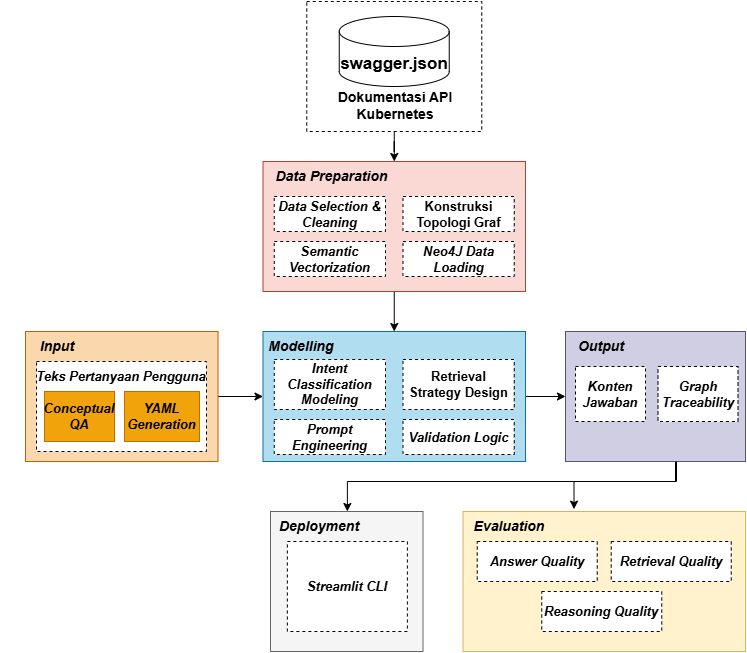
\includegraphics[width=1.00\textwidth]{images/Solusi-Methodology.png}
    \caption{Rancangan solusi berdasarkan metodologi CRISP--DM}
    \label{fig:crispdm_diagram}
\end{figure}

% ------------------------------------------------------------------
\section{Pemetaan Metodologi terhadap Kebutuhan Sistem}
% ------------------------------------------------------------------

Tahapan metodologi penelitian sebagaimana digambarkan pada Gambar~\ref{fig:crispdm_diagram}
menjadi landasan utama dalam perumusan kebutuhan sistem.
Setiap aktivitas pada tahap \textit{Data Preparation}, \textit{Modelling}, \textit{Input Processing},
\textit{Output Generation}, \textit{Evaluation}, dan \textit{Deployment} dipetakan secara langsung
terhadap kebutuhan fungsional yang harus dipenuhi oleh sistem.
Pemetaan ini memastikan bahwa rancangan solusi GraphRAG tidak hanya bersifat konseptual,
namun juga merefleksikan proses yang dibutuhkan untuk mencapai tujuan penelitian.
Hubungan antara tahapan metodologi dan kebutuhan fungsional ditunjukkan pada
Tabel~\ref{tbl:mapping_methodology_requirements}.

\renewcommand{\arraystretch}{1.35}
\captionsetup[longtable]{justification=raggedright,singlelinecheck=false}

\begin{longtable}{|p{3.8cm}|p{5cm}|p{4cm}|}
\caption{Pemetaan Tahap Metodologi}
\label{tbl:mapping_methodology_requirements} \\
\hline
\textbf{Tahap Metodologi} &
\textbf{Aktivitas Utama} &
\textbf{Kebutuhan yang Dipenuhi (F)} \\
\hline
\endfirsthead

\multicolumn{3}{l}{Tabel \ref{tbl:mapping_methodology_requirements} Pemetaan Tahap Metodologi (lanjutan)} \\
\hline
\textbf{Tahap Metodologi} &
\textbf{Aktivitas Utama} &
\textbf{Kebutuhan yang Dipenuhi (F)} \\
\hline
\endhead

\hline
\multicolumn{3}{r}{\textit{bersambung ke halaman berikutnya}} \\
\endfoot

\hline
\endlastfoot

% =================== DATA PREPARATION ======================
\multicolumn{3}{|c|}{\textbf{Data Preparation}} \\ \hline

\textit{Data Selection \& Cleaning} &
Identifikasi objek target dari spesifikasi OpenAPI Kubernetes, seleksi blok \textit{definitions}, dan pembersihan tipe generik yang tidak relevan untuk pembuatan YAML. &
F-01 (\textit{Structured Object Representation}),
F-05 (\textit{Semantic Embedding}) \\ \hline

Konstruksi Topologi Graf &
Transformasi struktur JSON menjadi node–edge dengan relasi referensial dan hierarkis. &
F-01 (\textit{Structured Object Representation}),
F-02 (\textit{Structured Relation Retrieval}),
F-05 (\textit{Semantic Embedding}) \\ \hline

\textit{Semantic Vectorization} &
Ekstraksi deskripsi objek menjadi \textit{embedding} numerik untuk pencarian semantik. &
F-05 (\textit{Semantic Embedding}) \\ \hline

Neo4j \textit{Data Loading} &
Memuat hasil konstruksi graf ke basis data Neo4j agar dapat ditelusuri kembali saat retrieval. &
F-01 (\textit{Structured Object Representation}) \\ \hline


% =================== MODELLING ======================
\multicolumn{3}{|c|}{\textbf{Modelling}} \\ \hline

\textit{Intent Classification Modeling} &
Klasifikasi pertanyaan pengguna ke dalam tipe \textit{intent} untuk menentukan strategi dan kedalaman penelusuran graf. &
F-03 (\textit{Intent Classification}) \\ \hline

\textit{Retrieval Strategy Design} &
Perancangan traversal graf berdasarkan entitas target, relasi, dan kebutuhan pengguna. &
F-02 (\textit{Structured Relation Retrieval}),
F-04 (\textit{Context Construction \& Injection}) \\ \hline

\textit{Prompt Engineering} &
Perancangan template \textit{prompt} untuk dua peran LLM serta injeksi konteks dan pengaturan format keluaran. &
F-04 (\textit{Context Construction \& Injection}),
F-07 (\textit{Conditional YAML Generation Constraint}) \\ \hline

\textit{Validation Logic} &
Integrasi prosedur validasi YAML bertingkat sebagai mekanisme \textit{fail-safe} yang memastikan keluaran memenuhi standar sintaksis, skema, dan kelengkapan \textit{field}. &
F-07 (\textit{Conditional YAML Generation Constraint}) \\ \hline

\textit{Conversation Memory Management} &
Penyimpanan dan pengambilan riwayat percakapan dalam \textit{pipeline} LangGraph untuk mendukung konteks \textit{multi-turn}. &
F-03 (\textit{Intent Classification}),
F-04 (\textit{Context Construction \& Injection}) \\ \hline


% =================== INPUT ======================
\multicolumn{3}{|c|}{\textbf{Input Processing}} \\ \hline

Pertanyaan Pengguna &
Input teks berupa permintaan teknis Kubernetes dalam bahasa alami yang diajukan pengguna melalui antarmuka percakapan. &
F-03 (\textit{Intent Classification}) \\ \hline


% =================== OUTPUT ======================
\multicolumn{3}{|c|}{\textbf{Output Generation}} \\ \hline

Konten Jawaban &
Keluaran sistem berupa narasi penjelas atau blok YAML konfigurasi Kubernetes sesuai permintaan pengguna. &
F-07 (\textit{Conditional YAML Generation Constraint}) \\ \hline

\textit{Graph Traceability} &
Penelusuran asal-usul \textit{field} melalui relasi \textit{node–edge} di dalam graf. &
F-02 (\textit{Structured Relation Retrieval}) \\ \hline


% =================== EVALUATION ======================
\multicolumn{3}{|c|}{\textbf{Evaluation}} \\ \hline

\textit{Answer Quality} (AnsQ) &
Evaluasi kualitas jawaban (\textit{Answer Quality}); definisi metrik lengkap pada Subbab~\ref{sec:metrik-evaluasi}. &
-- (Metrik domain, bukan requirement fungsional) \\ \hline

\textit{Retrieval Quality} (RetQ) &
Evaluasi kualitas \textit{retrieval} (\textit{Retrieval Quality}); definisi metrik lengkap pada Subbab~\ref{sec:metrik-evaluasi}. &
-- (Metrik domain, bukan requirement fungsional) \\ \hline

\textit{Reasoning Quality} (ReaQ) &
Evaluasi kualitas penalaran (\textit{Reasoning Quality}); definisi metrik lengkap pada Subbab~\ref{sec:metrik-evaluasi}. &
-- (Metrik domain, bukan requirement fungsional) \\ \hline


% =================== DEPLOYMENT ======================
\multicolumn{3}{|c|}{\textbf{Deployment}} \\ \hline

Antarmuka Web Interaktif (Streamlit) &
Penyajian sistem melalui antarmuka web berbasis Streamlit (\texttt{main.py}) yang menampilkan \textit{chat interface}, jawaban LLM, blok YAML (jika relevan), serta visualisasi \textit{Retrieval Trace} berbasis Graphviz. &
F-06 (\textit{Web Interaction Interface}) \\ \hline

\end{longtable}


Pemetaan pada Tabel~\ref{tbl:mapping_methodology_requirements} menunjukkan bahwa
seluruh tahapan metodologis yang digunakan dalam penelitian ini memiliki keterhubungan
langsung dengan kebutuhan fungsional yang dirancang. Setiap proses dalam
\textit{Data Preparation}, \textit{Modelling}, \textit{Input Processing},
\textit{Output Generation}, \textit{Evaluation}, dan \textit{Deployment}
telah diterjemahkan menjadi kapabilitas sistem yang operasional, terukur,
dan selaras dengan tujuan penelitian.
Rancangan masing-masing kebutuhan fungsional diuraikan secara terperinci pada
Subbab~\ref{sec:perancangan-kg} hingga Subbab~\ref{sec:perancangan-baseline}.

Untuk memberikan gambaran menyeluruh sebelum penjelasan detail tiap komponen,
Gambar~\ref{fig:architecture_diagram} menyajikan \textit{architecture diagram} yang
menggambarkan komponen sistem secara statis beserta keterhubungannya,
sedangkan Gambar~\ref{fig:sequence_diagram} menggambarkan alur interaksi antar-komponen
secara kronologis dari masukan pengguna hingga keluaran akhir.

\begin{figure}[H]
    \centering
    \captionsetup{justification=centering}
    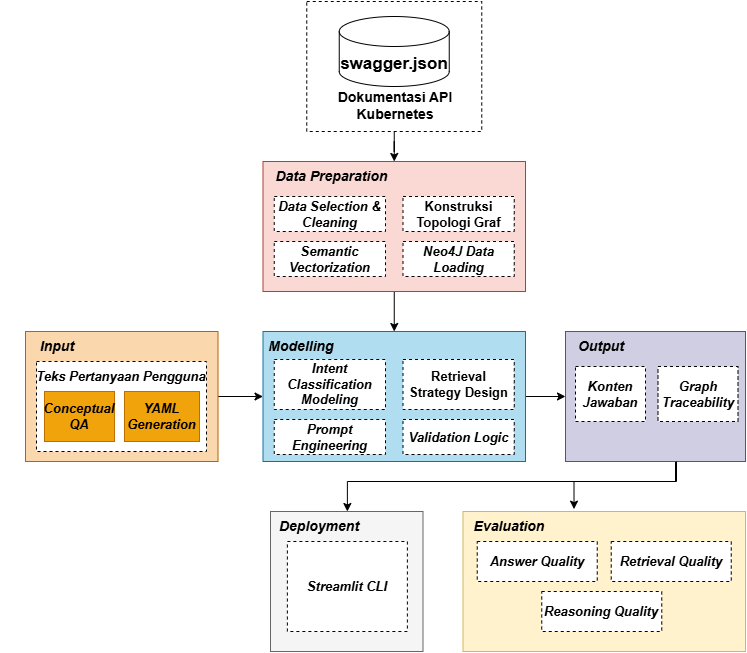
\includegraphics[width=1.00\textwidth]{images/Architecture.png}
    \caption{\textit{Architecture Diagram} Sistem \textit{GraphRAG} Kubernetes}
    \label{fig:architecture_diagram}
\end{figure}

\begin{figure}[H]
    \centering
    \captionsetup{justification=centering}
    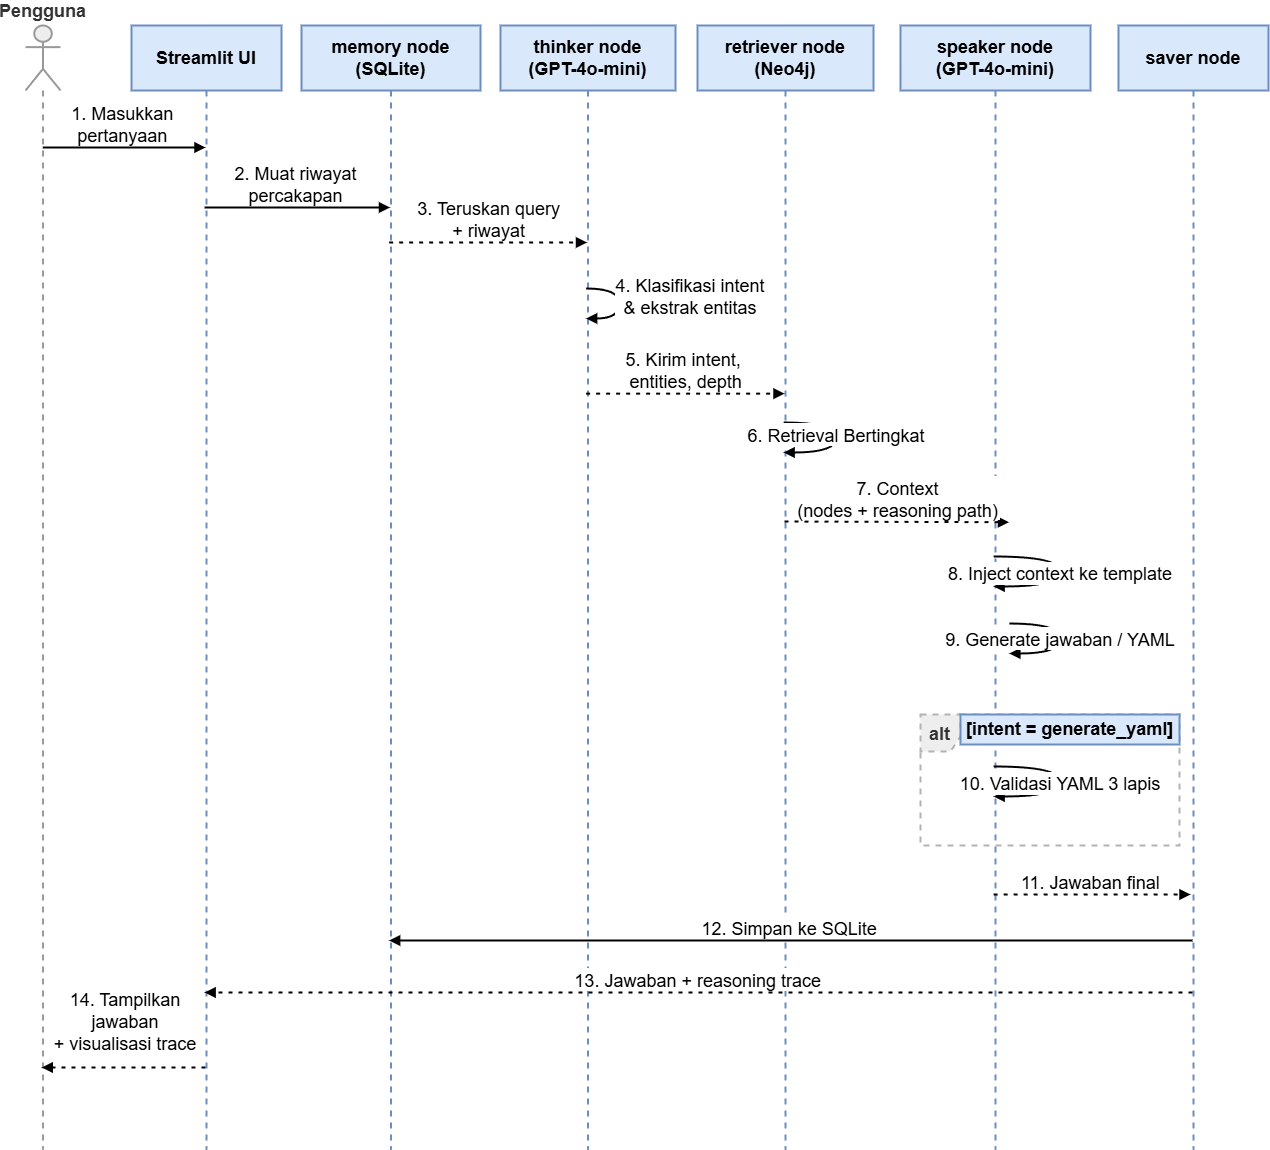
\includegraphics[width=1.00\textwidth]{images/Seq-High.png}
    \caption{Diagram Urutan (\textit{Sequence Diagram}) Alur Kerja Sistem GraphRAG}
    \label{fig:sequence_diagram}
\end{figure}

% ------------------------------------------------------------------
\section{Perancangan \textit{Knowledge Graph} Kubernetes}
\label{sec:perancangan-kg}
% ------------------------------------------------------------------

Kontribusi pertama penelitian ini, sebagaimana dirumuskan pada Bab~\ref{chap:pendahuluan},
adalah merancang \textit{pipeline} konstruksi \textit{knowledge graph} yang bersifat
deterministik berbasis skema OpenAPI Kubernetes (\textit{schema-derived deterministic KG construction}).
Graf dibangun langsung dari \texttt{swagger.json} melalui aturan transformasi yang eksplisit
sehingga hasil ekstraksi konsisten antar-eksekusi, berbeda dengan pendekatan berbasis LLM yang
menghasilkan struktur graf bervariasi karena bersifat stokastik.
Perancangan \textit{knowledge graph} mencakup tiga aspek yang saling melengkapi:
\begin{enumerate}
    \item \textit{pipeline ingestion} untuk representasi objek (F-01),
    \item strategi pembentukan relasi graf yang menjadi fondasi \textit{retrieval} (F-02), dan
    \item vektorisasi semantik untuk pencarian berbasis kemiripan (F-05).
\end{enumerate}

% --- 4.3.1 ---
\subsection{Perancangan \textit{Pipeline Ingestion} dan Representasi Objek}
\label{subsec:pipeline-ingestion}

\textit{Pipeline ingestion} bertanggung jawab memenuhi kebutuhan fungsional F-01
(\textit{Structured Object Representation}) dengan mengubah spesifikasi OpenAPI Kubernetes
(\textit{swagger.json}) menjadi \textit{knowledge graph} terstruktur yang tersimpan di Neo4j.
Proses ini dilaksanakan melalui lima \textit{pass} yang dieksekusi secara berurutan
sebagaimana ditunjukkan pada Gambar~\ref{fig:ingestion_pipeline}.

\begin{figure}[H]
    \centering
    \captionsetup{justification=centering}
    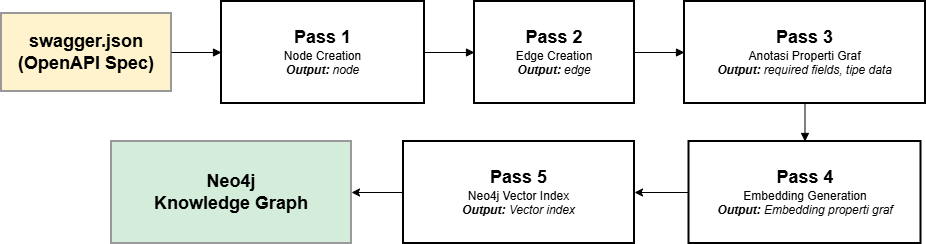
\includegraphics[width=0.50\textwidth]{images/ingestion_pipeline.png}
    \caption{Alur \textit{Pipeline Ingestion} dari \texttt{swagger.json} ke Neo4j \textit{Knowledge Graph}}
    \label{fig:ingestion_pipeline}
\end{figure}

Urutan \textit{pass} ini bersifat deterministik dan tidak dapat dibalik.

% --- 4.3.2 ---
\subsection{Perancangan Taksonomi Relasi \textit{Knowledge Graph}}
\label{subsec:edge-taxonomy}

Berdasarkan analisis pola keterhubungan data pada Bab~\ref{chap:analisis-masalah},
penelitian ini merancang strategi pembentukan relasi \textit{knowledge graph} yang
menggunakan dua mekanisme komplementer sebagaimana ditunjukkan pada
Tabel~\ref{tbl:strategi_relasi}.

\renewcommand{\arraystretch}{1.3}
\captionsetup[table]{justification=raggedright,singlelinecheck=false}
\begin{table}[H]
\caption{Strategi Pembentukan Relasi dalam \textit{Knowledge Graph} Kubernetes}
\label{tbl:strategi_relasi}
\centering
\begin{tabular}{|p{0.20\textwidth}|p{0.28\textwidth}|p{0.22\textwidth}|p{0.18\textwidth}|}
\hline
\textbf{Strategi} & \textbf{Sumber Derivasi} & \textbf{Contoh \textit{Edge}} & \textbf{Sifat} \\
\hline
Deterministik &
Referensi eksplisit \texttt{\$ref}, \texttt{allOf}, \texttt{oneOf}, \texttt{anyOf} dalam skema OpenAPI &
\textit{HAS\_PROPERTY}, \textit{EXTENDS}, \textit{ONE\_OF}, \textit{ANY\_OF} &
Konsisten 100\% antar-eksekusi \\
\hline
Semi-deterministik (berbasis aturan domain) &
Aturan transformasi berbasis semantik Kubernetes: pencocokan \textit{kind} dan pola jalur \textit{field} &
\textit{SELECTS\_POD}, \textit{BINDS\_ROLE}, \textit{SCALES\_RESOURCE}, \textit{MOUNTS\_VOLUME} &
Deterministik saat eksekusi. \\
\hline
\end{tabular}
\end{table}


Strategi pertama bersifat \textbf{deterministik}, yaitu setiap referensi \texttt{\$ref}, 
\texttt{allOf}, dan \texttt{oneOf},
\texttt{anyOf} dalam \texttt{swagger.json} diubah menjadi \textit{edge}.

Strategi kedua bersifat \textbf{semi-deterministik}, yaitu relasi yang tidak dinyatakan secara
eksplisit dalam skema OpenAPI tetapi relevan secara operasional di Kubernetes
(seperti relasi antara \textit{Service} dan \textit{Pod}, atau antara \textit{RoleBinding}
dan \textit{ServiceAccount}) dibentuk melalui aturan transformasi
berdasarkan semantik domain Kubernetes. Aturan ini bersifat deterministik saat dieksekusi
(hasil selalu sama untuk input yang sama), tetapi derivasi aturannya memerlukan pengetahuan
domain yang dienkode secara eksplisit.

% --- 4.3.3 ---
\subsection{Perancangan Vektorisasi Semantik}
\label{subsec:vektorisasi-semantik}

Vektorisasi semantik dirancang untuk memenuhi kebutuhan fungsional F-05
(\textit{Semantic Embedding}) dengan menghasilkan representasi vektor dari setiap node
dalam \textit{knowledge graph}. Vektor tersebut disimpan langsung sebagai properti setiap node di Neo4j, dan
sebuah indeks vektor dibangun agar pencarian kemiripan berbasis semantik dapat dieksekusi langsung dalam
graf yang sama tanpa memerlukan \textit{vector store} terpisah.

% ------------------------------------------------------------------
\section{Perancangan Mekanisme \textit{GraphRAG}}
\label{sec:perancangan-graphrag}
% ------------------------------------------------------------------

Kontribusi kedua penelitian ini, sebagaimana dirumuskan pada Bab~\ref{chap:pendahuluan},
adalah mengembangkan mekanisme GraphRAG dengan kedalaman \textit{traversal} yang disesuaikan
per tipe \textit{intent} (\textit{intent-adaptive depth traversal}).
Alih-alih menggunakan kedalaman tetap yang seragam, sistem menetapkan kedalaman berdasarkan
karakteristik struktural tiap jenis kueri sehingga \textit{retrieval} lebih presisi dan sesuai
dengan kebutuhan konteks.
Mekanisme ini juga mencakup validasi YAML berbasis \textit{knowledge graph}
serta antarmuka pengguna berbasis \textit{web} yang memungkinkan interaksi dalam bahasa alami.
Perancangan mekanisme GraphRAG terdiri dari empat komponen fungsional:
\begin{enumerate}
    \item klasifikasi \textit{intent} dan manajemen memori (F-03),
    \item strategi \textit{retrieval} bertingkat dan konstruksi konteks (F-02, F-04),
    \item generasi dan validasi YAML (F-07), serta
    \item antarmuka \textit{web} interaktif (F-06).
\end{enumerate}

% --- 4.4.1 ---
\subsection{Perancangan Klasifikasi \textit{Intent} dan Manajemen Memori}
\label{subsec:klasifikasi-intent}

Node \textit{thinker} bertanggung jawab memenuhi kebutuhan fungsional F-03
(\textit{Intent Classification}) melalui dua fungsi utama: (1) mengklasifikasikan maksud
dari kueri pengguna, dan
(2) mengekstrak entitas Kubernetes yang disebutkan dalam kueri.
\textit{Node thinker} menghasilkan keluaran berformat JSON menggunakan konfigurasi deterministik. 
Hal ini bertujuan agar klasifikasi \textit{intent} dan ekstraksi entitas tetap konsisten setiap kali 
kueri yang identik dieksekusi.

jenis \textit{intent} dibedakan berdasarkan jenis informasi yang dibutuhkan dan kedalaman traversal yang sesuai.
Kedalaman yang lebih besar ditetapkan untuk tipe \textit{intent} yang memerlukan konteks
relasional lebih luas, sedangkan kedalaman yang lebih kecil ditetapkan untuk kueri yang
bersifat spesifik.

Manajemen memori percakapan dirancang menggunakan basis data relasional ringan dengan
identifikasi sesi berbasis UUID. Pada setiap interaksi, riwayat percakapan dimuat dan
diteruskan ke node \textit{thinker} bersama kueri baru.
Riwayat ini memungkinkan komunikasi 2 arah antara LLM dengan pengguna, contohnya untuk memahami rujukan seperti "hal tersebut" atau "itu" berdasarkan konteks percakapan
sebelumnya tanpa memerlukan pengulangan nama entitas secara eksplisit.
Setelah respons dihasilkan, pasangan kueri-respons disimpan untuk digunakan pada
interaksi berikutnya.

% --- 4.4.2 ---
\subsection{Perancangan Strategi \textit{Retrieval} dan Konstruksi Konteks}
\label{subsec:retrieval-bertingkat}

Node \textit{retriever} mengimplementasikan \textit{cascading retrieval} dengan tiga tahap
berurutan untuk memenuhi kebutuhan fungsional F-02 (\textit{Structured Relation Retrieval})
dan F-04 (\textit{Context Construction \& Injection}).

\begin{enumerate}
    \item \textbf{Tahap 1: \textit{Exact Name Match} (Prioritas Utama).} \\
    Sistem mencari \textit{node} pada Neo4j yang namanya sama persis dengan entitas hasil ekstraksi 
    \textit{node thinker}. Jika ditemukan, \textit{node} ini akan dijadikan sebagai \textit{seed node} 
    (simpul awal) untuk penelusuran graf. Pendekatan ini memberikan presisi tertinggi karena 
    mengandalkan pencocokan eksak, bukan sekadar perkiraan semantik.

    \item \textbf{Tahap 2: \textit{Vector Similarity} (\textit{Fallback}).} \\
    Tahap ini hanya dieksekusi apabila Tahap 1 tidak menemukan kecocokan. Sistem akan menghasilkan 
    representasi vektor dari kueri pengguna, kemudian mencari \textit{node} dengan tingkat kemiripan 
    tertinggi menggunakan indeks vektor pada Neo4j. Kandidat dengan skor kemiripan terbesar tersebut 
    selanjutnya digunakan sebagai \textit{seed node}.

    \item \textbf{Tahap 3: \textit{Multi-hop Graph Traversal}.} \\
    Berawal dari \textit{seed node}, sistem melakukan penelusuran graf pada Neo4j secara rekursif. 
    Batas kedalaman penelusuran disesuaikan dengan jenis \textit{intent} dari kueri. Penentuan 
    kedalaman ini didasarkan pada distribusi karakteristik \textit{node} di masing-masing level, 
    sebagaimana dirangkum pada Tabel~\ref{tbl:hop_justification}.
\end{enumerate}

\renewcommand{\arraystretch}{1.3}
\captionsetup[table]{justification=raggedright,singlelinecheck=false}
\begin{table}[H]
\caption{Distribusi karakteristik \textit{node} berdasarkan kedalaman penelusuran graf}
\label{tbl:hop_justification}
\centering
\begin{tabular}{| c | p{0.20\textwidth} | p{0.30\textwidth} | p{0.25\textwidth} |}
\hline
\textbf{Kedalaman} & \textbf{Karakteristik \textit{Node}} & \textbf{Contoh} & \textbf{Penggunaan} \\
\hline
1--2 & Spesifik \textit{resource} (dibagikan 2--3 \textit{resource}) & \textit{DeploymentSpec}, \textit{ServiceSpec} & Tipe \textit{explain}, \textit{followup} \\
\hline
3 & \textit{Field} tingkat kontainer & \textit{image}, \textit{ports}, \textit{env}, \textit{resources} & Tipe \textit{generate\_yaml}, \textit{trace\_relationship} \\
\hline
4+ & Tipe generik (dibagikan 19--136 \textit{resource}) & \textit{Quantity}, \textit{IntOrString}, \textit{LocalObjectReference} & \textbf{Tidak digunakan} (menurunkan presisi) \\
\hline
\end{tabular}
\end{table}


Tabel~\ref{tbl:hop_justification} menunjukkan bahwa karakteristik \textit{node} berubah secara
signifikan seiring bertambahnya kedalaman: \textit{node} pada kedalaman 1--2 bersifat spesifik
terhadap \textit{resource}, sedangkan \textit{node} pada kedalaman 4 ke atas merupakan tipe
generik yang dibagikan oleh 19--136 \textit{resource} sehingga menurunkan presisi konteks.
Kedalaman traversal dibatasi pada rentang 2--3 untuk menghindari injeksi tipe generik yang
tidak informatif ke dalam konteks LLM.

Setelah traversal selesai, node \textit{retriever} membangun \textit{reasoning path} berupa
daftar relasi dengan format \texttt{Parent -[REL]-> Child} yang merepresentasikan jalur
relasional yang dilalui selama traversal.
Konteks yang terbentuk dari \textit{reasoning path} beserta riwayat percakapan kemudian
diinjeksikan ke dalam \textit{prompt template} yang diteruskan ke node \textit{speaker}
sebagai bukti penalaran yang dapat dilihat oleh pengguna.

% --- 4.4.3 ---
\subsection{Perancangan Generasi dan Validasi YAML}
\label{subsec:perancangan-yaml}

Node \textit{speaker} bertanggung jawab memenuhi kebutuhan fungsional F-07
(\textit{Conditional YAML Generation Constraint}) melalui dua jalur keluaran yang
ditentukan secara kondisional berdasarkan tipe \textit{intent}.
Apabila \textit{intent} diklasifikasikan sebagai \textit{generate\_yaml}, sistem menghasilkan
blok kode YAML konfigurasi Kubernetes yang kemudian divalidasi melalui mekanisme
validasi tiga lapis.
Apabila \textit{intent} bukan \textit{generate\_yaml}, sistem menghasilkan jawaban naratif
tanpa proses validasi YAML.

Validasi YAML tiga lapis ini dirancang sebagai
\textit{KG-grounded structural validation}.
Berbeda dengan pendekatan \textit{dry-run} yang memerlukan klaster Kubernetes aktif,
validasi lapis ketiga dilakukan langsung terhadap \textit{knowledge graph} yang telah
dibangun pada tahap \textit{ingestion} sehingga verifikasi \textit{required fields}
dapat dilakukan tanpa menggunakan infrastruktur Kubernetes langsung.
Ketiga lapis validasi dieksekusi secara berurutan sebagaimana ditunjukkan pada
Gambar~\ref{fig:yaml_validation}.

\begin{figure}[H]
    \centering
    \captionsetup{justification=centering}
    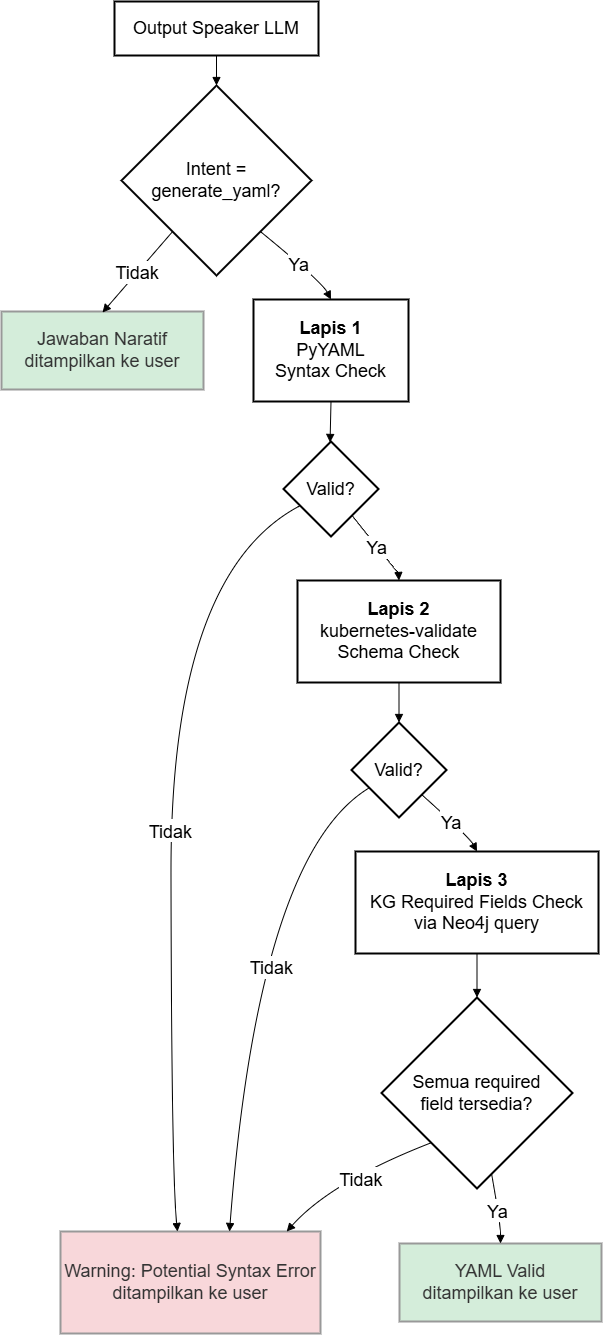
\includegraphics[width=0.85\textwidth]{images/yaml_validation.png}
    \caption{Alur Validasi YAML Tiga Lapis Berbasis \textit{Knowledge Graph}}
    \label{fig:yaml_validation}
\end{figure}

% --- 4.4.4 ---
\subsection{Perancangan Antarmuka \textit{Web} Interaktif}
\label{subsec:perancangan-antarmuka}

Antarmuka \textit{web} interaktif dirancang untuk memenuhi kebutuhan fungsional F-06
(\textit{Web Interaction Interface}) sebagai \textit{entry point} utama sistem GraphRAG.
Gambar~\ref{fig:usecase_diagram} menggambarkan empat interaksi utama yang dapat dilakukan
pengguna dengan sistem dalam bentuk \textit{use case diagram}.

\begin{figure}[H]
    \centering
    \captionsetup{justification=centering}
    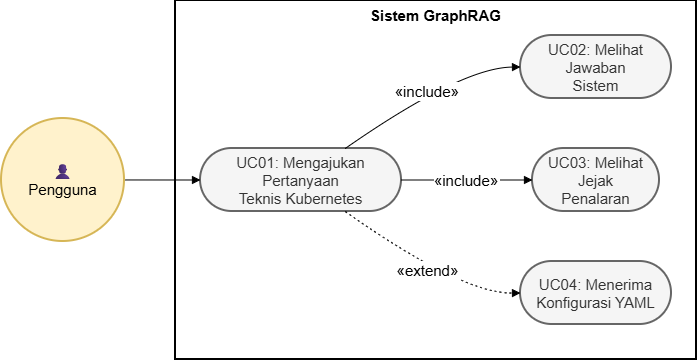
\includegraphics[width=0.85\textwidth]{images/UseCase.png}
    \caption{\textit{Use Case Diagram} Interaksi Pengguna dengan Sistem GraphRAG}
    \label{fig:usecase_diagram}
\end{figure}

Antarmuka menyediakan tiga komponen utama.
Pertama, \textit{chat interface} sebagai sarana masukan pertanyaan dalam bahasa alami.
Kedua, area keluaran yang menampilkan jawaban naratif atau blok YAML konfigurasi
beserta peringatan validasi apabila relevan.
Ketiga, \textit{Retrieval Trace Expander} yang menyajikan jejak penalaran graf dalam empat tab:
\begin{enumerate}
    \item visualisasi Graphviz yang menampilkan \textit{reasoning path} secara grafis;
    \item tabel relasi \textit{node} yang dilalui selama traversal;
    \item referensi resmi \textit{kubernetes.io} untuk setiap entitas yang ditemukan; dan
    \item legenda kedalaman traversal.
\end{enumerate}

% ------------------------------------------------------------------
\section{Perancangan Sistem Pembanding}
\label{sec:perancangan-baseline}
% ------------------------------------------------------------------

Untuk memenuhi tujuan ketiga penelitian ini (T3), ditetapkan dua sistem pembanding
(\textit{baseline}) yang digunakan dalam evaluasi komparatif pada Bab~\ref{chap:evaluasi}.
Penetapan sistem pembanding yang terdefinisi dengan baik merupakan prasyarat untuk
menghasilkan perbandingan yang adil (\textit{fair comparison}): ketiga sistem menggunakan
model LLM yang sama (GPT-4o-mini) dan dataset uji yang sama (97 \textit{fixture}),
sehingga perbedaan kinerja dapat diatribusikan pada mekanisme \textit{retrieval},
bukan pada kapabilitas model.

Ketiga sistem yang dibandingkan membentuk rangkaian evolusi yang progresif:
Vector RAG menyempurnakan Vanilla LLM dengan menambahkan mekanisme \textit{retrieval}
berbasis kemiripan semantik, sedangkan GraphRAG menyempurnakan Vector RAG dengan
menambahkan traversal graf \textit{multi-hop}, klasifikasi \textit{intent},
dan validasi YAML berbasis \textit{knowledge graph}.

% --- 4.5.1 ---
\subsection{Evolusi Rancangan Ketiga Sistem}
\label{subsec:evolusi-rancangan}

Gambar~\ref{fig:evolusi_sistem} menggambarkan evolusi komponen ketiga sistem secara berlapis.
Komponen dasar yang digunakan bersama oleh ketiga sistem ditampilkan pada lapisan pertama.
Komponen yang ditambahkan oleh Vector RAG ditampilkan pada lapisan kedua, sedangkan
komponen tambahan yang hanya dimiliki GraphRAG ditampilkan pada lapisan ketiga.

\begin{figure}[H]
    \centering
    \captionsetup{justification=centering}
    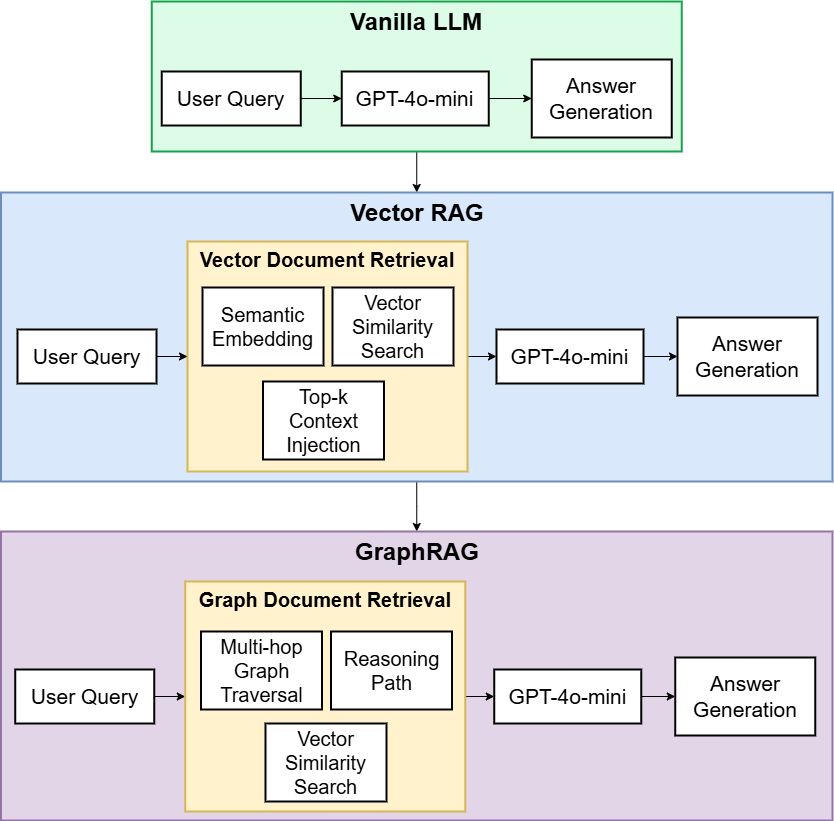
\includegraphics[width=0.80\textwidth]{images/Evolusi-Sistem.png}
    \caption{Evolusi Rancangan: Vanilla LLM $\rightarrow$ Vector RAG $\rightarrow$ GraphRAG}
    \label{fig:evolusi_sistem}
\end{figure}

% --- 4.5.2 ---
\subsection{Rancangan Vanilla LLM}
\label{subsec:rancangan-vanilla}

Vanilla LLM menggunakan GPT-4o-mini secara langsung tanpa mekanisme \textit{retrieval}
apapun. Pertanyaan pengguna diteruskan langsung ke model tanpa konteks tambahan sehingga
jawaban bergantung sepenuhnya pada pengetahuan parametrik model.
Alur pemrosesan bersifat langsung: kueri pengguna $\rightarrow$ GPT-4o-mini
$\rightarrow$ jawaban.
Sebagai kondisi dasar tanpa proses augmentasi, sistem ini digunakan sebagai acuan batas bawah kinerja untuk evaluasi komparatif antara ketiga sistem.

% --- 4.5.3 ---
\subsection{Rancangan Vector RAG}
\label{subsec:rancangan-vector-rag}

Vector RAG menggunakan \textit{retrieval} berbasis kemiripan \textit{embedding} atas
indeks vektor Neo4j. Kueri pengguna di-\textit{embed} menggunakan model yang sama dengan
GraphRAG, kemudian digunakan untuk mencari \textit{node} paling mirip (top-$k$=5)
dengan ekspansi satu lompatan ke \textit{node} tetangga.
Konteks hasil \textit{retrieval} diteruskan ke GPT-4o-mini sebagai \textit{speaker}.
Alur pemrosesan adalah: kueri pengguna $\rightarrow$ \textit{embedding}
$\rightarrow$ pencarian vektor (top-$k$=5) $\rightarrow$ ekspansi 1 lompatan
$\rightarrow$ konstruksi konteks $\rightarrow$ GPT-4o-mini $\rightarrow$ jawaban.
Sistem ini merepresentasikan pendekatan RAG konvensional tanpa
\textit{intent-adaptive multi-hop traversal}.

% --- 4.5.4 ---
\subsection{Rangkuman Perbandingan Komponen Teknis}
\label{subsec:perbandingan-komponen}

Tabel~\ref{tbl:perbandingan_sistem} merangkum perbedaan komponen teknis ketiga sistem
yang dibandingkan. Perbedaan komponen ini menjadi dasar interpretasi hasil evaluasi
pada Bab~\ref{chap:evaluasi}: peningkatan kinerja yang konsisten dari Vanilla LLM ke
Vector RAG dan dari Vector RAG ke GraphRAG mengindikasikan kontribusi masing-masing
komponen tambahan terhadap aspek kualitas yang diukur.

\renewcommand{\arraystretch}{1.3}
\captionsetup[table]{justification=raggedright,singlelinecheck=false}
\begin{table}[H]
\caption{Perbandingan Komponen Teknis Ketiga Sistem}
\label{tbl:perbandingan_sistem}
\centering
\begin{tabular}{|p{0.22\textwidth}|p{0.20\textwidth}|p{0.22\textwidth}|p{0.24\textwidth}|}
\hline
\textbf{Aspek} & \textbf{Vanilla LLM} & \textbf{Vector RAG} & \textbf{GraphRAG} \\
\hline
Metode \textit{retrieval} &
Tidak ada (pengetahuan parametrik) &
Kemiripan vektor (top-$k$=5) &
\textit{Exact match} $\rightarrow$ vektor $\rightarrow$ \textit{multi-hop traversal} \\
\hline
Sumber konteks &
--- &
Neo4j Vector Index (1 lompatan) &
Neo4j \textit{Knowledge Graph} (2--3 lompatan) \\
\hline
Kedalaman traversal &
--- &
Tetap (1 lompatan) &
Adaptif per \textit{intent} (kedalaman 2--3) \\
\hline
Klasifikasi \textit{intent} &
--- &
--- &
5 tipe \textit{intent} (F-03) \\
\hline
Validasi YAML &
--- &
--- &
Tiga lapis: sintaksis, skema, \textit{KG} (F-07) \\
\hline
Manajemen memori &
--- &
--- &
SQLite (riwayat percakapan) \\
\hline
Kebutuhan fungsional &
--- &
F-05 (parsial) &
F-01 s.d. F-07 (lengkap) \\
\hline
\end{tabular}
\end{table}
